% !TeX root = relazione.tex
\documentclass{article}

\usepackage[utf8]{inputenc}
\usepackage[a4paper, total={15.3 cm, 21.3 cm}]{geometry}
\usepackage{amsmath}
\usepackage{amssymb}
\usepackage{gensymb}
\usepackage{booktabs}
\usepackage{hyperref}
\usepackage{caption}
\usepackage{float}
\usepackage{graphicx}
\usepackage{subfig}
\usepackage{titlesec}
\usepackage{titletoc}
\usepackage{physics}
\usepackage{siunitx}
\usepackage[dvipsnames]{xcolor}

\usepackage{longtable}
\usepackage{tabularx}
\usepackage{calc}
\usepackage{array}
\usepackage{subfiles}
\usepackage{etoolbox}
\usepackage{xparse}


\hypersetup{colorlinks=true,linkcolor=black}
\renewcommand\thesection{\arabic{section}}
\titlecontents{chapter}[1.05em]{\bigskip}
{\contentslabel[\MakeUppercase{\romannumeral\thecontentslabel}]{1em}\enspace\textsc}
{\hspace*{-1em}\textsc}
{\hfill\contentspage}
\titlecontents{section}[1.6em]{\smallskip}
{\thecontentslabel.\enspace}
{}
{\titlerule*[1pc]{.}\contentspage}
\setcounter{tocdepth}{2}


\begin{document}

    \pagenumbering{roman}
    \thispagestyle{empty}

    % First page with uni logo and title
    \begin{center}

        
\includegraphics[width=1.\linewidth]{../../tools/images/logo.jpg}
        \centering
        \vspace{3cm}

        \uppercase{\Large Relazione di laboratorio:\\ Misura della velocità della luce \par}
        \vspace{3cm}

        \Large Lorenzo Liuzzo, Jiahao Miao, Riccardo Salto\par
        \vspace{1.5cm}

        \Large Ottobre 26, 2022

    \end{center}

    \clearpage

    % Table of contents
    \tableofcontents

    \clearpage
    \pagenumbering{arabic}

    % Abstract con una breve descrizione dell'esperimento e i risultati
    \section{Abstract}

        L'obbiettivo dell'esperimento è la misura della velocità della luce in aria. 
        Riproducendo l'esperimento di Focault, è stato ricavato indirettamente il seguente risultato: 
        \[ c = (2.94 \pm 0.22) \cdot 10^8 \, \mathrm{m/s} \] compatibile entro 0.3 $\sigma$ dal valore noto.

    \section{Metodi}

        La misura della velocità della luce ha avuto luogo attraverso due fasi principali: la calibrazione dell'apparato e l'effettiva misurazione 
        delle grandezze fisiche utili al calcolo della velocità della luce.

        \subsection{Calibrazione dell'apparato}

            Innanzitutto è stata verificato il corretto posizionamento del laser attraverso la squadretta forata con precisione di qualche millimetro. 
            Si è osservata una leggera ($1 \qq*{mm}$ c.ca) inclinazione verso l'alto che è stata considerata trascurabile. 
            Dopodiché, è stato posizionato lo specchio rotante verso il laser per controllarne l'auto-collimazione, 
            confermando la trascurabilità dell'inclinazione di cui sopra. 
            Una volta posizionate le due lenti $L_1$ e $L_2$, di rispettiva focale $F_1 = 48$ mm, $F_2= 252$ mm, 
            a distanza $D_1= 70$ mm, $D_2=378$ mm dall'uscita del raggio, esse sono state regolate in modo tale da centrare il foro della squadretta. 
            Si è proseguito col posizionamento del canotto porta-cannocchiale con splitter integrato, verificando che il fascio di ritorno fosse riflesso 
            al centro del canotto, intercettando il laser tramite un foglio semi-trasparente di carta millimetrata appoggiatovi sopra. 
            Le regolazioni sono state effettuate con il micrometro e la levetta dello splitter.
            
            Agendo sulla cinghia di trasmissione dello specchio rotante è stato direzionato il fascio verso il primo specchio piano $S_1$, 
            che è stato regolato affinchè il raggio ne puntasse il centro, facendolo scorrere sul carrello al quale è stato assicurato. 
            Si è osservato un leggero abbassamento del raggio causato dal passaggio attraverso lo splitter. 
            Regolando l'inclinazione di $S_1$ con le viti micrometriche si è puntato il raggio verso il centro del secondo specchio piano $S_2$, 
            a sua volta regolato in modo tale che il fascio entrasse nel centro dello specchio concavo $MF$. 
            Attraverso minime correzioni nel posizionamento di $L_2$ (effettuate segnando la larghezza del pallino per diverse disposizioni, 
            data la difficoltà nel far strisciare la lente con continuità sulla rotaia), la cui posizione finale era $D_f=380$ mm, 
            si è minimizzato lo spessore dello spot luminoso. Tramite la regolazione delle viti micrometriche è stato reindirizzato il fascio di ritorno 
            in modo da farlo collimare con il raggio di andata. 
            Quando la collimazione è avvenuta con buona approssimazione, il fascio è comparso sulla parte bianca del porta-specchio-rotante e 
            nel canotto del cannocchiale su cui era appoggiato il foglio di carta millimetrata. Da qui in poi è stato più semplice centrare lo spot luminoso. 
            La procedura si è svolta in modo relativamente veloce e senza grosse complicazioni.
            
            E' tuttavia risultato più complicato l'inserimento del cannocchiale, poiché non si riusciva a localizzare lo spot luminoso. 
            Dunque, dopo una serie  di regolazioni senza risultato, si è pensato che lo splitter potesse essere stato montato al contrario. 
            Ne è stata quindi invertita l'inclinazione e l'apparato è stato completamente ricalibrato. 
            A questo punto si è capito che il problema non fosse quello e si è tornati alla configurazione iniziale, ripetendo di nuovo tutte le procedure. 
            Con difficoltà è stato finalmente osservato lo spot luminoso nel cannocchiale: l'apparato era dunque pronto per effettuare le misurazioni. 
        

        \subsection{Misure distanze specchi}

            Per prima cosa sono state misurate le distanze tra specchio rotante e primo specchio piano $MR-S_1$, tra i due specchi piani $S_1-S_2$, 
            ed infine tra il secondo specchio piano e lo specchio concavo $S_2-MF$. 
            Si è scelto di fare queste misurazioni dopo la calibrazione per limitarne l'errore, già piuttosto pesante nella misura finale, 
            nonostante fosse facile perdere la calibrazione del sistema. \\
            Riportiamo di seguito la figura \ref{fig:apparato} che mostra lo schema dell'apparato sperimentale e 
            la tabella \ref{tabular:distanze} che riporta le misure delle distanze degli specchi. \\

            \begin{figure}[H]

                \centering
                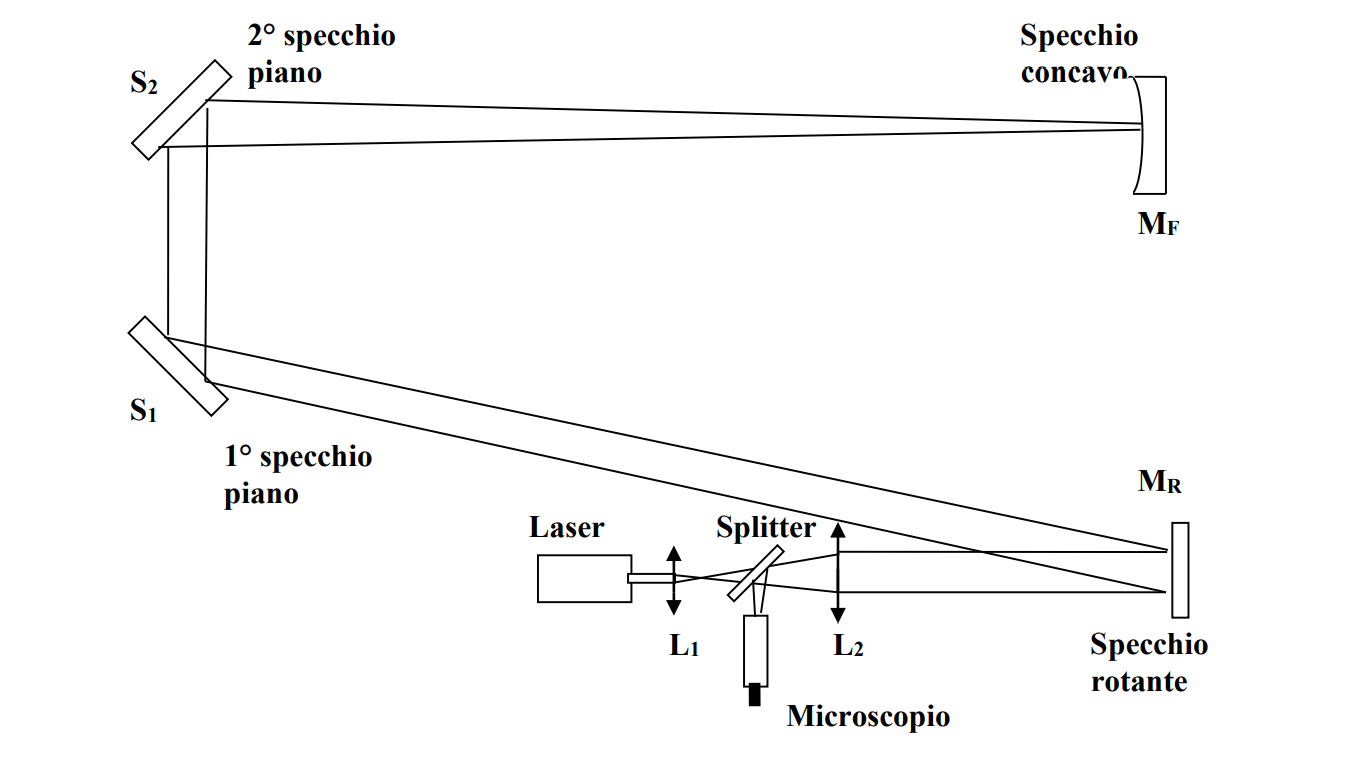
\includegraphics[width=8cm]{../images/apparato.png}

                \captionof{figure}{Schema dell'apparato sperimentale}
                \label{fig:apparato}
                
            \end{figure}

            \begin{table}[H]

                \centering

                \begin{tabular}{ c c c } 
                        
                    \toprule
                    \textbf{Segmento} & D [m] & $\sigma_D$ [m] \\ 

                    \midrule
                        $MR-S1$     &   6.26    & 0.01  \\ 
                        $S_1-S_2$   &   0.58    & 0.01  \\ 
                        $S_2-MF$    &   6.47    & 0.01  \\ 
                    \bottomrule                

                \end{tabular}

                \captionof{table}{Misure distanze specchi}
                \label{tabular:distanze}

            \end{table}
        

        \subsection{Misure Clock-Wise}
            
            Le prime misure effettuate sono state quelle in cui lo specchio ruotava in senso orario. 
            Sono state osservate la frequenza di rotazione dello specchio a basso regime ($\nu < 300 $ Hz) leggendola dallo strumento con risoluzione 1 Hz e 
            la relativa posizione dello spot luminoso con il micrometro di risoluzione 0.01 mm, e, in seguito, 
            la frequenza di rotazione ad alto regime ($\nu > 750 $ Hz) e la relativa posizione dello spot. 
            Nella tabella \ref{tabular:rawdataCW}, sono riportate le misure delle frequenze iniziali e finali insieme alle relative posizioni angolari. \\

            \begin{table}[H]

                \centering
                \begin{tabular}{c c c c c c c c} 

                    \toprule
                    $\nu_0$ [Hz] & $\sigma_{\nu_0}$ [Hz] & $\nu_f$ [Hz] &  $\sigma_{\nu_f}$ [Hz] & 
                    $\delta_0$ [mm] & $\sigma_{\delta_0}$ [mm] & $\delta_f$ [mm] & $\sigma_{\delta_f}$ [mm] \\ 
                    
                    \midrule
                        193 & 5 & 738   & 5 & 9.18 & 0.05 & 9.00 & 0.05  \\ 
                        156 & 5 & 878   & 5 & 9.19 & 0.05 & 8.96 & 0.05  \\ 
                        126 & 5 & 747   & 5 & 9.22 & 0.05 & 9.02 & 0.05  \\ 
                        132 & 5 & 787   & 5 & 9.17 & 0.05 & 8.98 & 0.05  \\ 
                        213 & 5 & 882   & 5 & 9.18 & 0.05 & 8.97 & 0.05  \\ 
                        100 & 5 & 1450  & 5 & 9.22 & 0.05 & 8.83 & 0.05  \\ 
                        106 & 5 & 880   & 5 & 9.25 & 0.05 & 8.97 & 0.05  \\ 
                        294 & 5 & 811   & 5 & 9.17 & 0.05 & 8.96 & 0.05  \\ 
                        160 & 5 & 758   & 5 & 9.19 & 0.05 & 8.92 & 0.05  \\ 
                        289 & 5 & 1390  & 5 & 9.16 & 0.05 & 8.76 & 0.05  \\ 
                        355 & 5 & 823   & 5 & 9.14 & 0.05 & 8.93 & 0.05  \\ 
                        104 & 5 & 740   & 5 & 9.20 & 0.05 & 8.97 & 0.05  \\ 
                        251 & 5 & 816   & 5 & 9.19 & 0.05 & 8.97 & 0.05  \\ 
                        268 & 5 & 880   & 5 & 9.18 & 0.05 & 8.93 & 0.05  \\ 
                        82  & 5 & 1380  & 5 & 9.17 & 0.05 & 8.78 & 0.05  \\ 
                        35  & 5 & 880   & 5 & 9.17 & 0.05 & 8.94 & 0.05  \\ 
                        28  & 5 & 905   & 5 & 9.17 & 0.05 & 8.73 & 0.05  \\ 
                        96  & 5 & 776   & 5 & 9.25 & 0.05 & 8.97 & 0.05  \\ 
                        118 & 5 & 880   & 5 & 9.23 & 0.05 & 8.91 & 0.05  \\ 
                        174 & 5 & 1350  & 5 & 9.20 & 0.05 & 8.67 & 0.05  \\ 
            
                    \bottomrule           
                
                \end{tabular}

                \caption{Dati misure Clock-Wise}
                \label{tabular:rawdataCW}

            \end{table}
            
            Sono state fatte le omogenee differenze tra le due misure che sono state utilizzate per ricavare la velocità della luce e la sua incertezza
            dalle formule:  
            \[ c= \frac{4Df_2\Delta\omega}{(D+a-f_2)\Delta\delta} \]
            \[ \sigma_c = c \cdot \sqrt{(\frac{(D + 2a - 2f_2) \cdot \sigma_D}{(D + a - f_2) \cdot D})^2 + 
                        (\frac{\sigma_a}{D + a - f_2})^2 + (\frac{\sigma_\omega}{\omega})^2 + (\frac{\sigma_\delta}{\delta})^2}
            \label{propagazione err luce} \] \\
            
            Per prima cosa si è osservato che a basse frequenze lo spot luminoso si trovava al limite dello spostamento del cannocchiale con il micrometro. 
            Un'osservazione che sul momento non è parsa rappresentare un problema, ma col senno del poi probabilmente ha influito 
            nell'errore sistematico riscontato nel set di misure, dalle quali la velocità della luce media risulta essere:    
            \[ c_{cw} = (2.3 \pm 0.7)\cdot10^8 \, \mathrm{m/s} \] 

            Si è poi scelto di non effettuare misurazioni nel range 300-750 Hz poiché a quelle frequenze la cinghia slittava leggermente e 
            il valore di frequenza osservato era palesemente diverso dal valore reale. 
            Inoltre una massimizzazione di $\Delta \omega$ ne avrebbe minimizzato l'errore relativo.
            Riportiamo nella tabella \ref{tabular:dati c} i dati osservati e nella figura \ref{fig:c_CW} la loro rappresentazione grafica.
        
            \begin{minipage}{\textwidth}

                \begin{minipage}[b]{0.35\textwidth}

                    \centering
                    \begin{tabular}{c c} 
                        
                        \toprule
                        c [m/s] &  $\sigma_c$ [m/s] \\ 
                        \midrule
                        2.50E+08	&    1.00E+08 \\
                        2.60E+08	&    0.80E+08 \\
                        2.60E+08	&    0.90E+08 \\
                        2.64E+08	&    0.90E+08 \\
                        2.90E+08	&    0.50E+08 \\
                        2.90E+08	&    1.00E+08 \\
                        2.30E+08	&    0.60E+08 \\
                        2.30E+08	&    0.80E+08 \\
                        2.00E+08	&    0.50E+08 \\
                        2.30E+08	&    0.40E+08 \\
                        1.90E+08	&    0.60E+08 \\
                        2.30E+08	&    0.70E+08 \\
                        2.10E+08	&    0.70E+08 \\
                        2.00E+08	&    0.60E+08 \\
                        2.80E+08	&    0.50E+08 \\
                        3.00E+08	&    1.00E+08 \\
                        1.70E+08	&    0.30E+08 \\
                        2.00E+08	&    0.50E+08 \\
                        2.00E+08	&    0.40E+08 \\
                        1.90E+08	&    0.30E+08 \\
                        \bottomrule

                    \end{tabular}
                    
                    \captionof{table}{Set di misure della velocità della luce}
                    \label{tabular:dati c}

                \end{minipage}
                \begin{minipage}[b]{0.65\linewidth}  

                    \centering
                    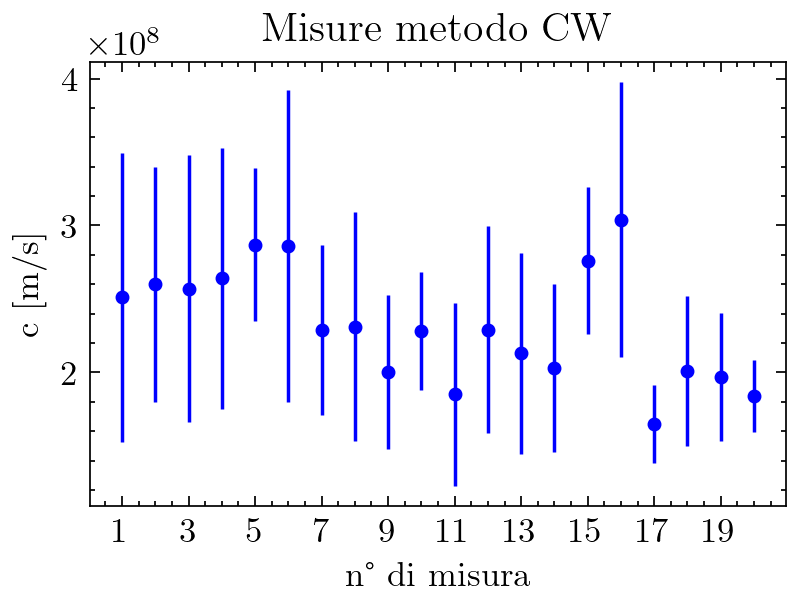
\includegraphics[width=10cm]{../images/CW.png}

                    \captionof{figure}{Misure CW}
                    \label{fig:c_CW}

                \end{minipage}
            
            \end{minipage}
            
            
        \subsection{Misure Counter-Clock-Wise}

            Per la presa dati di frequenze e posizioni si è proceduto con lo stesso modus operandi descritta sopra. 
            In questa fase è stato riscontrato ripetute volte la scomparsa improvvisa dello spot luminoso, in particolare per frequenze elevate. 
            In seguito a un'altra serie di controlli e ricalibrazioni, si è giunti alla conclusione che ciò fosse dovuto principalmente all'intensità del fondo 
            troppo luminoso rispetto alla luce fioca del laser al ritorno. 
            Dopo la quinta misura è stato perso definitivamente lo spot luminoso. È quindi stato necessario riposizionare il canotto porta-cannocchiale e 
            ricalibrare la strumentazione (le distanze tra i componenti sono risultate le medesime).
            Questa variazione porta con sé cambiamenti nelle misure delle posizioni pressochè irrilevanti, dato l'utilizzo degli spostamenti relativi dello spot.
            Riportiamo di seguito i dati osservati e la loro rappresentazione grafica.   

            \begin{table}[H]

                \centering
                \begin{tabular}{c c c c c c c c} 

                    \toprule
                    $\nu_0$ [Hz] & $\sigma_{\nu_0}$ [Hz] & $\nu_f$ [Hz] &  $\sigma_{\nu_f}$ [Hz] & 
                    $\delta_0$ [mm] & $\sigma_{\delta_0}$ [mm] & $\delta_f$ [mm] & $\sigma_{\delta_f}$ [mm] \\ 
                    
                    \midrule
                    104 & 5 & 862 &  5 & 9.20 & 0.05 & 8.98 & 0.05  \\ 
                    77  & 5 & 878 &  5 & 9.23 & 0.05 & 8.96 & 0.05  \\ 
                    128 & 5 & 774 &  5 & 9.17 & 0.05 & 8.91 & 0.05  \\
                    183 & 5 & 890 &  5 & 9.20 & 0.05 & 8.95 & 0.05  \\ 
                    244 & 5 & 820 &  5 & 9.16 & 0.05 & 8.93 & 0.05  \\ 
                    59  & 5 & 790 &  5 & 8.76 & 0.05 & 8.96 & 0.05  \\ 
                    101 & 5 & 775 &  5 & 9.17 & 0.05 & 8.90 & 0.05  \\ 
                    217 & 5 & 810 &  5 & 8.79 & 0.05 & 8.96 & 0.05  \\ 
                    124 & 5 & 853 &  5 & 8.76 & 0.05 & 8.99 & 0.05  \\ 
                    170 & 5 & 865 &  5 & 8.77 & 0.05 & 8.97 & 0.05  \\ 
                    232 & 5 & 876 &  5 & 8.78 & 0.05 & 8.99 & 0.05  \\ 
                    256 & 5 & 807 &  5 & 8.77 & 0.05 & 8.93 & 0.05  \\ 
                    291 & 5 & 803 &  5 & 8.79 & 0.05 & 8.95 & 0.05  \\ 
                    308 & 5 & 847 &  5 & 8.76 & 0.05 & 8.95 & 0.05  \\ 
                    136 & 5 & 1424 & 5 & 8.77 & 0.05 & 9.12 & 0.05  \\ 
                    \bottomrule           
                
                \end{tabular}
                \caption{Dati misure Counter-Clock-Wise}

            \end{table}

            \begin{table}[H]

                \begin{minipage}{0.35\linewidth}

                    \centering
                    \begin{tabular}{ c c } 

                        \toprule
                        c [m/s] &  $\sigma_c$ [m/s] \\ 

                        \midrule
                        3E+08	&    1E+08 \\
                        2.5E+08	&    7E+07 \\
                        2.0E+08	&    6E+07 \\
                        2.3E+08	&    6E+07 \\
                        2.1E+08	&    6E+07 \\
                        3E+08	&    1E+08 \\
                        2.1E+08	&    5E+07 \\
                        3E+08	&    1E+08 \\
                        2.6E+08	&    8E+07 \\
                        3E+08	&    1E+08 \\
                        2.6E+08	&    9E+07 \\
                        3E+08	&    1E+08 \\
                        3E+08	&    1E+08 \\
                        2.4E+08	&    9E+07 \\
                        3.1E+08	&    6E+07 \\
                        \bottomrule 

                    \end{tabular}
                    \caption{raw data CCW}
    
                \end{minipage}
                \begin{minipage}{0.65\linewidth}

                    \centering
                    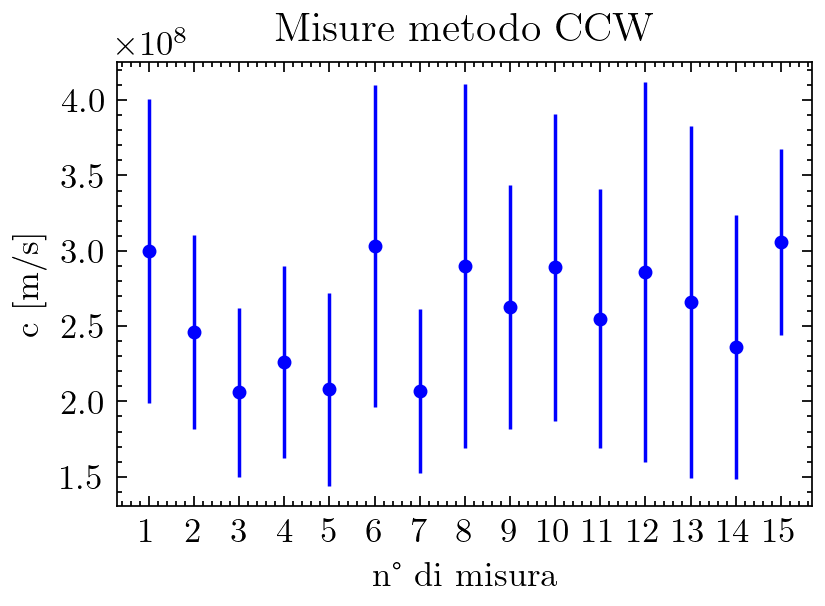
\includegraphics[width=10cm]{../images/CCW.png}
                    \captionof{figure}{Misure CCW}
                    \label{fig:c_CCW}

                \end{minipage}
                
            \end{table}

            La stima migliore di c ottenuta in questa fase è: \[ c_{ccw} = (2.6 \pm 0.9)\cdot10^8 \, \mathrm{m/s} \] 
         
        
        \subsection{Misure CW-CCW}

            In questa fase è stata modificata la procedura di presa dati per massimizzare l'escursione delle frequenze di rotazione dello specchio. 
            Le misure sono state infatti ottenute facendo ruotare lo specchio a frequenze elevate prima in senso orario, poi antiorario. 
            Data la mancanza di tempo sono state prese solo tre misure, che sono risultate essere le più accurate. 
            
            Riportiamo di seguito i dati osservati e la loro rappresentazione grafica.
            
            \begin{table}[H]

                \centering
                \begin{tabular}{c c c c c c c c} 

                    \toprule
                    $\nu_0$ [Hz] & $\sigma_{\nu_0}$ [Hz] & $\nu_f$ [Hz] &  $\sigma_{\nu_f}$ [Hz] & 
                    $\delta_0$ [mm] & $\sigma_{\delta_0}$ [mm] & $\delta_f$ [mm] & $\sigma_{\delta_f}$ [mm] \\ 
                    
                    \midrule
                    1410 & 20 & -1426 & 20 & 8.34 & 0.03 & 9.12 & 0.03  \\ 
                    879 & 10 & -862 & 10 & 8.49 & 0.03 & 8.96 & 0.03  \\ 
                    800 & 10 & -833 & 10 & 8.53 & 0.03 & 8.97 & 0.03  \\ 
                    \bottomrule           
                
                \end{tabular}

                \caption{Dati misure CW-CCW}

            \end{table}

            \begin{table}[H]
                
                \centering
                \begin{minipage}{0.35\linewidth}

                    \centering
                    \begin{tabular}{ c c }
                        
                        \toprule
                        c [m/s] &  $\sigma_c$ [m/s] \\
                        
                        \midrule
                        3.00E+08 & 0.20E+08  \\
                        3.10E+08 & 0.30E+08  \\ 
                        3.10E+08 & 0.30E+08  \\
                        \bottomrule 

                    \end{tabular}

                    \caption{Set di misure della velocità della luce CW-CCW}

                \end{minipage}
                \begin{minipage}{0.6\linewidth}

                    \centering
                    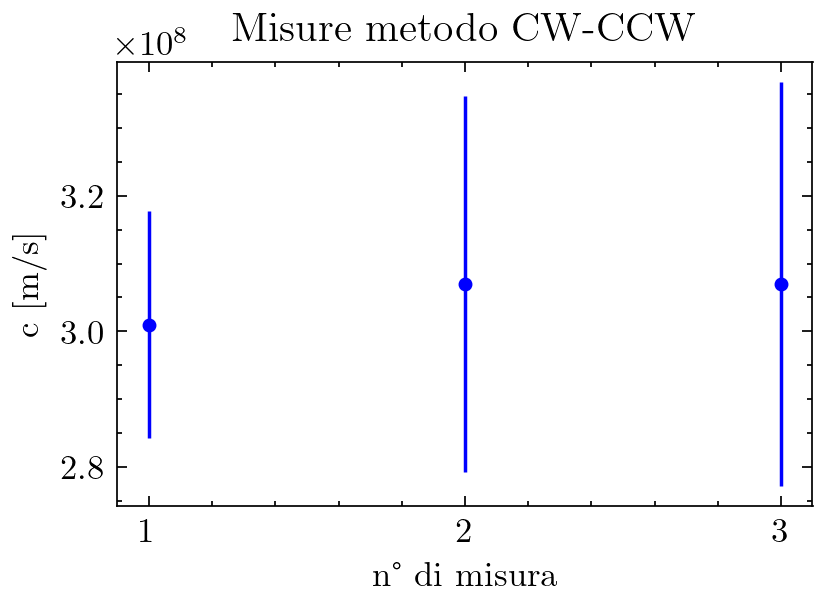
\includegraphics[width=10cm]{../images/CW_CCW.png}

                    \captionof{figure}{Misure CW-CCW}

                \end{minipage}

            \end{table}

            La stima migliore di c ottenuta è di : \[c_{cw} = (3.0	\pm 0.3) \cdot 10^8 \, \mathrm{m/s}\] 
        
        \newpage


    \section{Analisi dati}
    
        Per l'analisi dati, si presuppone di non conoscere il valore "vero" della velocità della luce. \\
        Dalle venti misure CW, sono state ricavate altrettante misure di c con i relativi errori calcolati propagando le incertezze 
        con la formula \ref{propagazione err luce}, da cui osserviamo che l'incertezza è direttamente proporzionale al valore calcolato, 
        come si può osservare nei grafici \ref{fig:c_CW} e \ref{fig:c_CCW}. 
        Una media ponderata è stata considerata poco efficiente in quanto l'errore ottenuto è risultato poco credibile (in quanto "piccolo"). 
        Si è poi osservato che veniva dato così peso a misure molto poco precise e accurate. Inoltre si è osservato che a basse frequenze 
        lo spot luminoso variava di molto poco la sua posizione, quindi valutare l'errore in modo diverso per ogni misura non pareva sensato.
        Si è perciò optato per una media aritmetica dei 20 valori come miglior valore e come incertezza la somma in quadratura tra 
        la media aritmetica delle incertezze e la deviazione standard della media $\frac{\sigma}{\sqrt{N}}$, 
        in modo da tenere conto della dispersione fra i valori e avere un errore abbastanza omogeneo. \\

        La stessa analisi è stata eseguita per i valori CCW e CW-CCW, ottenendo i valori migliori per le varie modalità di misura, 
        valori che sono riportati alla fine dei rispettivi paragrafi e nel seguente grafico. 
        
        \begin{figure}[H]

            \centering
            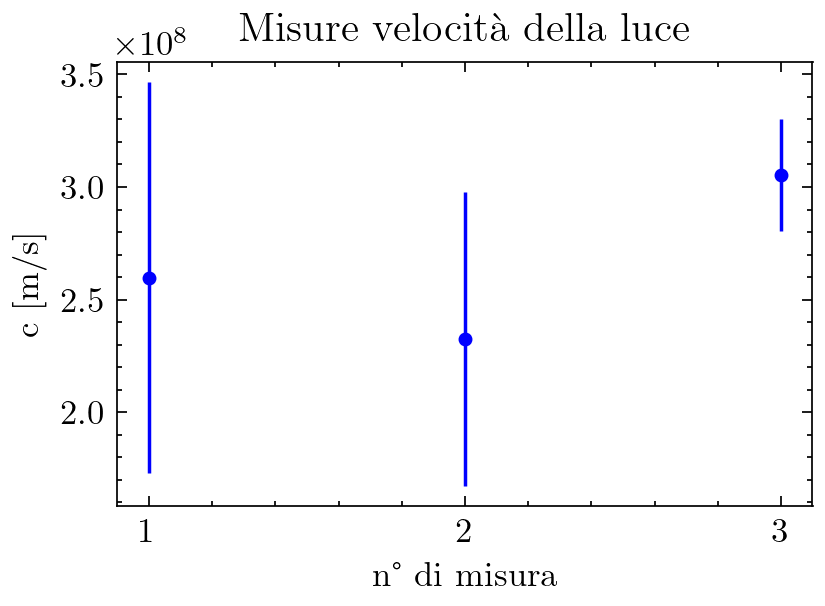
\includegraphics[width=10cm]{../images/results.png}
            \caption{Confronto misure}

        \end{figure}

        In ultima istanza, di questi tre valori  è stata fatta la media pesata ottenendo così il valore finale: 
        \[ c_{best} = (2.9 \pm 0.2)\cdot10^8 \, \mathrm{m/s}. \]
        Confrontando tale valore con il valore nominale ($ c = 299 792 458$ m/s) diviso per l'indice di rifrazione dell'aria ($ n_{aria} = 1.00029$), 
        si osserva che il valore misurato è compatibile entro $0.3 ~\sigma$ dal valore noto. 

    \newpage


    \section{Considerazioni finali}

        Durante il corso delle prime misurazioni si sono presentate una serie di complicazioni nella calibrazione dello strumento e 
        pertanto nel corso dell'intera sessione di laboratorio è stato necessario eseguire più correzioni, quali persino il riposizionamento del canotto e 
        ricalibrazione dello strumento. Per questo motivo si è scelto di analizzare in modo indipendente i set di dati ottenuti con le differenti modalità illustrate 
        nelle sezioni precedenti. Riportiamo di seguito un grafico dei valori ottenuti rispetto alle misurazioni effettuate, comparate col valore accetto.
            
        \begin{figure}[H]
            \centering
            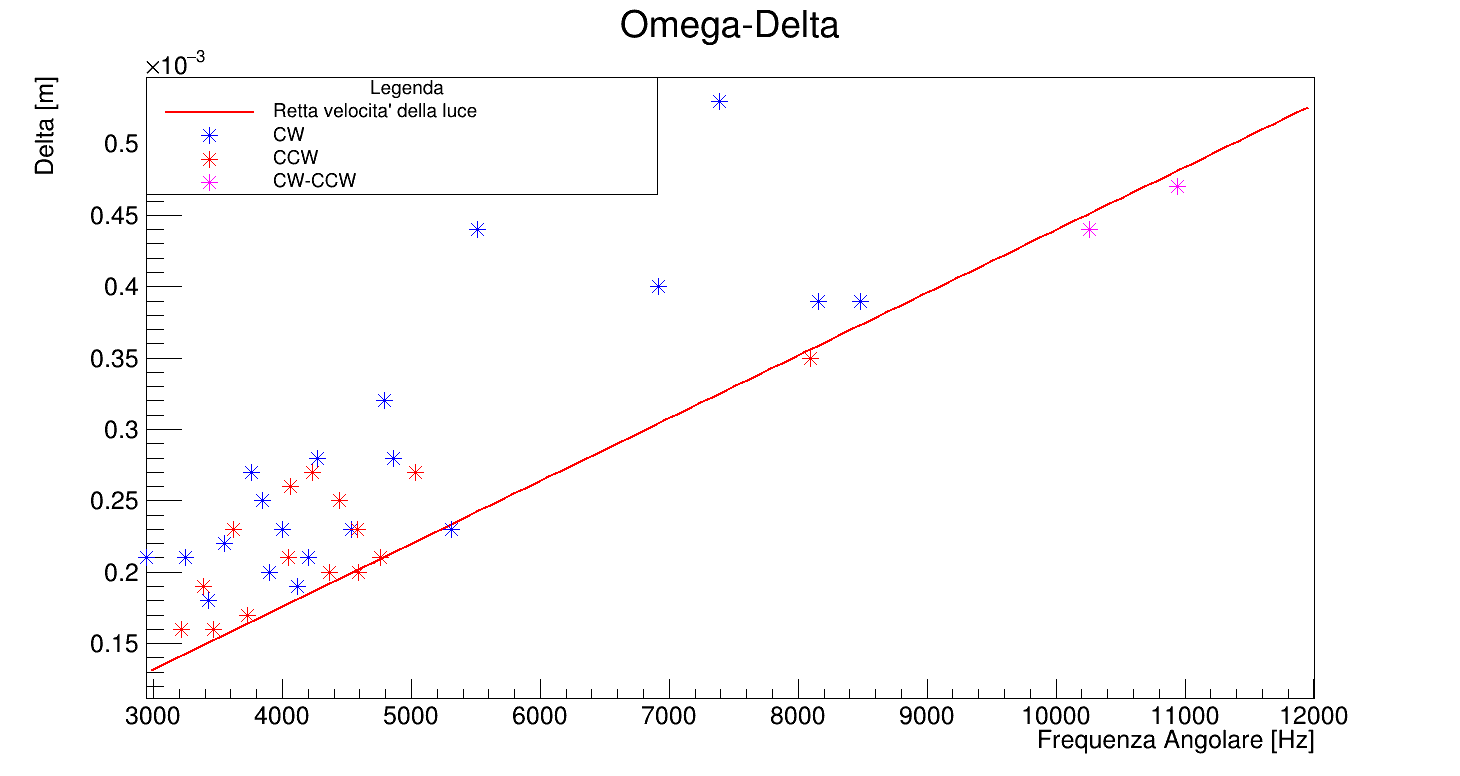
\includegraphics[scale=0.32]{../images/omega_delta1.png}
            \caption{Grafico $\Delta\omega-\Delta\delta$}
            \label{fig:Omega-Delta}
        \end{figure}
        
        La figura \ref{fig:Omega-Delta} rappresenta una proiezione in piano della funzione velocità:
        \[ v(\Delta \omega,\Delta \delta)= \frac{4Df_2\Delta\omega}{(D+a-f_2)\Delta\delta} \]
        La retta {\color{Red}rossa} è la funzione definita implicitamente da $v(\Delta \omega,\Delta \delta)= c$, da ciò si può dedurre che 
        le curve di livello a velocità costante sono delle rette parallele a quella in figura. 
        Nel grafico si osserva immediatamente che la maggioranza dei punti si collocano al di sopra della retta, 
        ciò è indice del fatto che le misure sono affette da errore sistematico.

        Si nota che il set di misurazioni CW presenta maggiore dispersione, indice di minore precisione ed è inoltre meno accurato. 
        Invece, il set CWW presenta alcune misure molto accurate mentre altre più disperse, però tutte distribuite secondo delle rette parallele a quella nota. 
        Le misurazioni CW e alcune di quelle CWW sono state effettuate prima della ricalibrazione dello strumento. 
        Inoltre, se si osservano solo quelle effettuate dopo, risulta palese che la ricalibrazione ha diminuito l'errore sistematico.

        \begin{figure}[H]

            \centering
            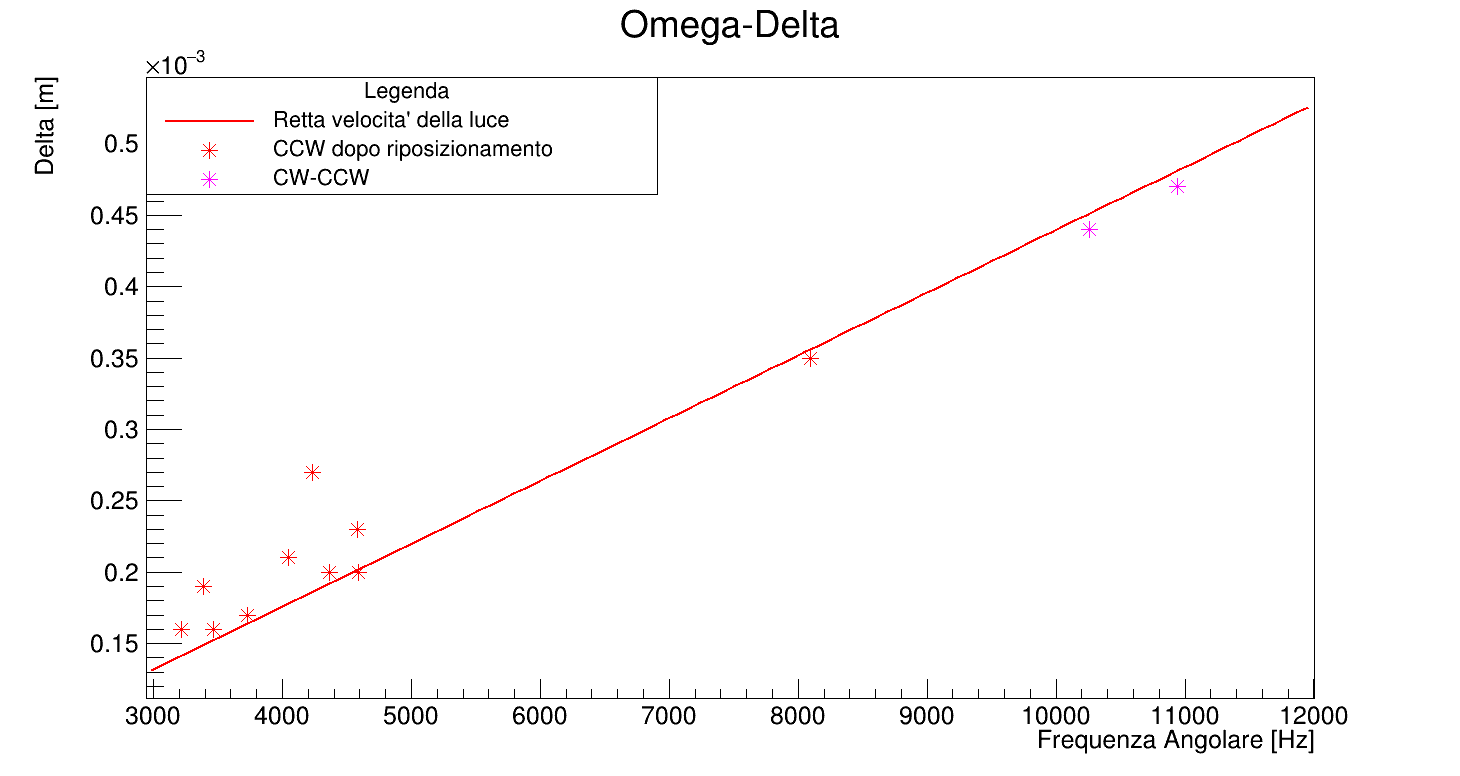
\includegraphics[scale=0.32]{../images/omega_delta2.png}
            \caption{Grafico $\Delta\omega-\Delta\delta$ dopo il riposizionamento}
            \label{fig:Omega-Delta2}

        \end{figure}

        Si può infatti facilmente notare che le misurazioni escluse erano quelle più lontane dalla retta. 
        Il valore della velocità che si ottiene con questo set di dati ripulito è 
        $c_{clean} = (3.0 \pm 0.2) \cdot 10^8\, \mathrm{m/s}$, rispetto al valore calcolato precedente mediando tra i valori ottenuti dai diversi set di misure, 
        pari a $c_{best} = (2.9 \pm 0.2)\cdot10^8\, \mathrm{m/s.}$
        Confrontando tali valori con il valore nominale ($ c = 299 792 458\, \mathrm{m/s}$) diviso per l'indice di rifrazione dell'aria ($n_{aria} = 1.00029$), 
        è possibile affermare che i valori trovati sono rispettivamente entro i $0.1~\sigma$ e  $0.3~\sigma$ dal valore noto.


\end{document}